\begin{figure}[ht]
    \centering
    \begin{subfigure}[t]{0.47\linewidth}
        \centering
        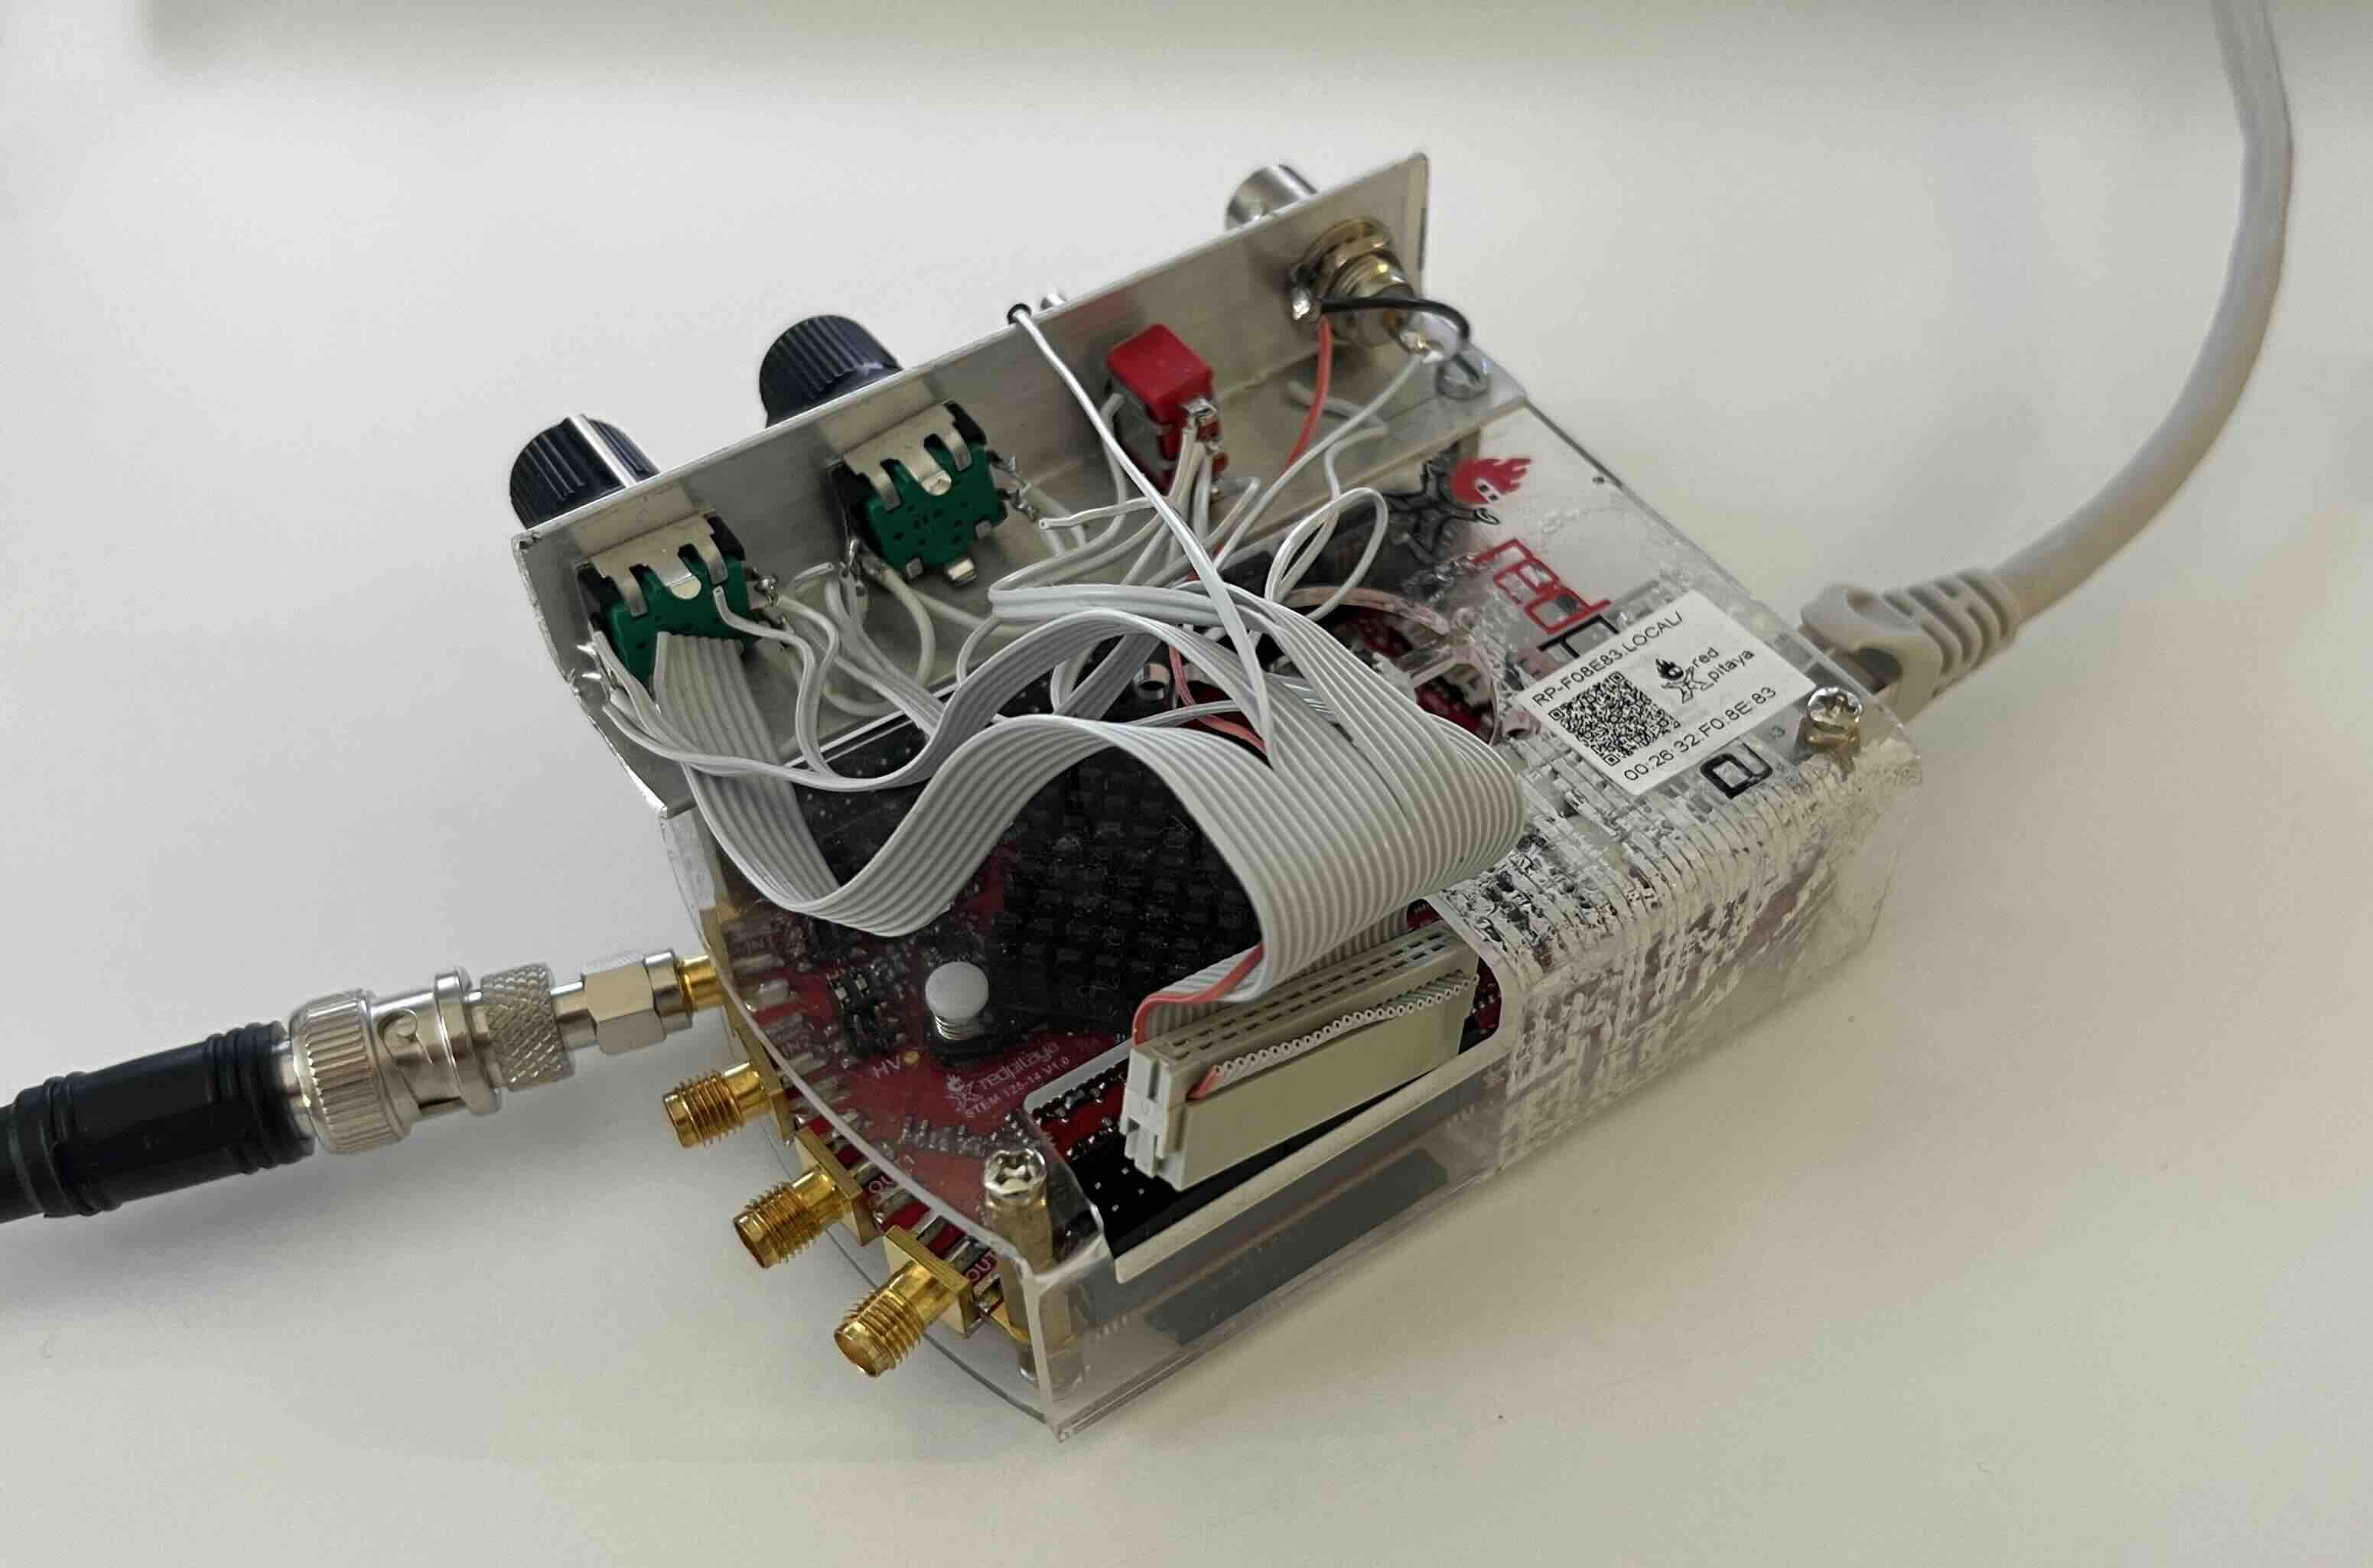
\includegraphics[width=\textwidth]{images/chapter_2/red_pitaya.jpeg}
        \caption{Red Pitaya STEMlab 125-14 model single-board computer.}
        \label{fig:ch2_red_pitaya}
    \end{subfigure}
    \hspace{.025\linewidth}
    \begin{subfigure}[t]{0.47\linewidth}
        \centering
        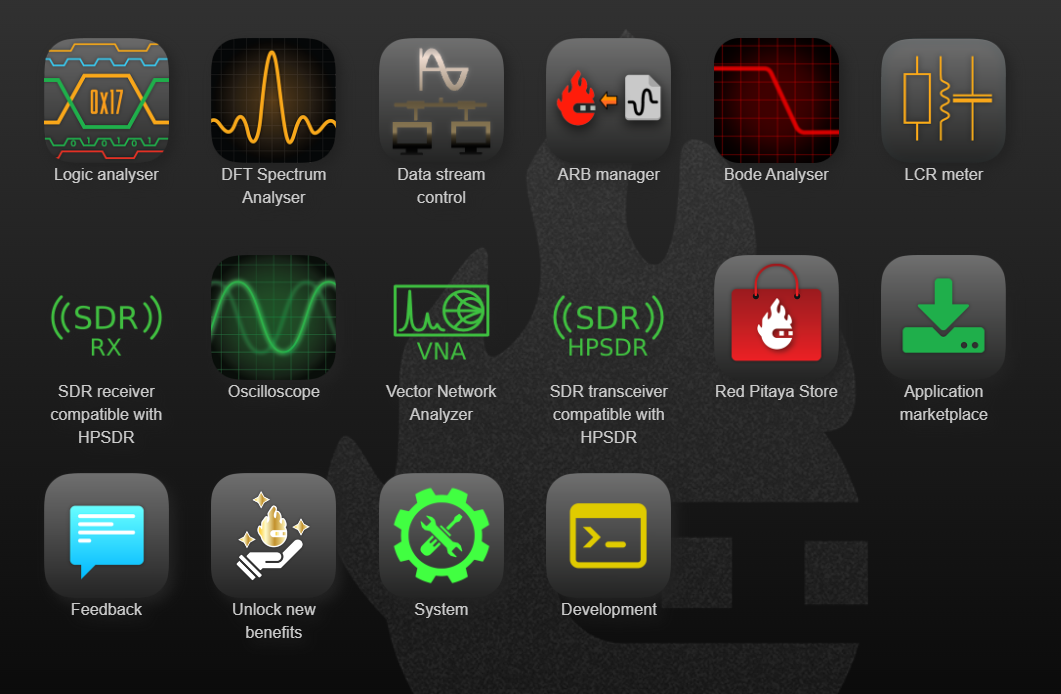
\includegraphics[width=\textwidth]{images/chapter_2/rp_apps.png}
        \caption{Red Pitaya web homepage interface with default applications.}
        \label{fig:ch2_rp_apps}
    \end{subfigure}
    \caption{The Red Pitaya.}
    \label{fig:ch1_lenses_cavity}
\end{figure}

\noindent Red Pitaya is a single-board computer first created to be an alternative for various expensive laboratory equipments for control measurements. The experiment uses the STEMlab 125-14 model running on ecosystem version 1.04. The model includes a Xilinx system-on-chip (SoC) with a CPU and an FPGA, two 125 MS/s inputs and two 125 MS/s outputs coupled with 14-bit analog-to-digital (ADC) and digital-to-analog (DAC) converters, ethernet connectivity, and more. The Red Pitaya is well known for its proprietary hardware design and open-source software development framework. By default, the Red Pitaya can function as an oscilloscope, an LCR meter, a spectrum analyzer, logic analyzer, and so on \cite{rp}. For the experiment, we wish to exploit Red Pitaya's 125 MS/s inputs coupled to the ADC, which could replace the NI 5761 Analog Input module for data acquisition purposes.

Some key specifications for the Red Pitaya STEMlab 125-14 and the NI 5761 Analog Input modules are listed in Table \ref{tab:rp_ni}. Although the STEMlab 125-14 has less analog inputs and a slower sampling rate than the NI 5761, it is significantly less costly, such that needing multiple modules to compensate is still economically practical.

\begin{table}[h!]
    \centering
    \begin{tabular}{ p{5cm} | p{6cm} | p{5cm} }
        \hline
        \textbf{Key Specifications} & \textbf{Red Pitaya STEMlab 125-14}
            & \textbf{NI 5761 Analog Input} \\
        \hline
        Number of Inputs & 2 & 4 \\
        ADC Sampling Rate & 125 MHz & 250 MHz \\
        ADC Resolution & 14-bit & 14-bit \\
        ADC Range & $\pm$1 V (LV) and $\pm$20 V (HV) & $\pm$1 V \\
        Price & \euro\ 465,60 & \euro\ 4.500,00 \\
        \hline
    \end{tabular}
    \caption{Key specifications for the Red Pitaya STEMlab 125-14 and the NI 5761 Analog Input modules.}
    \label{tab:rp_ni}
\end{table}

To get started with STEMlab 125-14, I followed the introductory tutorials provided by Red Pitaya. The tutorials covered the basics of hardware and software programming associated with the Red Pitaya, which differs from that of the Digilent Cmod A7, as the Red Pitaya is much more complex. Following this, I moved onto exploring whether the Red Pitaya could satisfy key experimental requirements, which include sufficient memory storage for data acquisition, input noise limits, and discontinuous data acquisition.

%%%%%%%%%%%%%%%%%%%%%%%%%%%%%%%%%%%%%%%%%%%%%%%%%%%%%%%%%%%%%%%%%%%%%%%%%%%%%%%%
\subsection{Input Data Memory Storage \& Extension}\label{2_3_1_memory}
\subfile{subsections/2_3_1_memory}

%%%%%%%%%%%%%%%%%%%%%%%%%%%%%%%%%%%%%%%%%%%%%%%%%%%%%%%%%%%%%%%%%%%%%%%%%%%%%%%%
\subsection{Input Noise}\label{2_3_1_noise}
\subfile{subsections/2_3_2_noise}

%%%%%%%%%%%%%%%%%%%%%%%%%%%%%%%%%%%%%%%%%%%%%%%%%%%%%%%%%%%%%%%%%%%%%%%%%%%%%%%%
\subsection{Discontinuous Acquisition}\label{2_3_1_discon_acq}
\subfile{subsections/2_3_3_discon_acq}
